% Made up for the tikra benchmark.
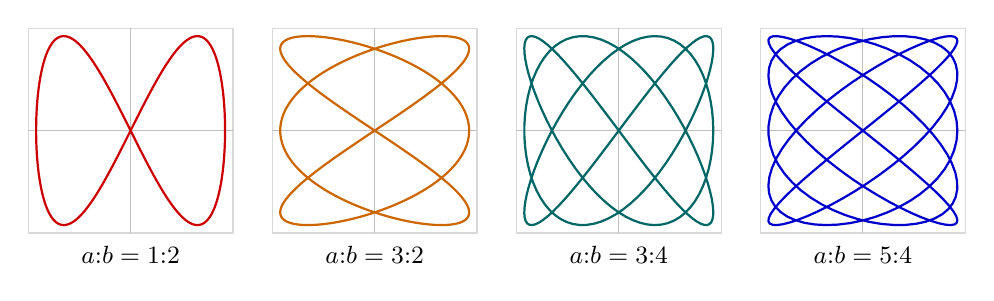
\begin{tikzpicture}[line join=round]
  \foreach \a/\b/\c [count=\i from 0] in {1/2/red, 3/2/orange, 3/4/teal, 5/4/blue} {
    \begin{scope}[xshift=\i*3.1cm]
      \draw[gray!30] (-1.3,-1.3) rectangle (1.3,1.3);
      \draw[gray!50] (-1.3,0) -- (1.3,0) (0,-1.3) -- (0,1.3);
      \draw[\c!80!black, thick, domain=0:360, samples=240, variable=\t]
        plot ({1.2*sin(\a*\t + 90)}, {1.2*sin(\b*\t)});
      \node[below, font=\small] at (0,-1.35) {$a{:}b = \a{:}\b$};
    \end{scope}
  }
\end{tikzpicture}
